\documentclass{beamer}
\usepackage{amsmath}
\usepackage{hyperref}
\usepackage{listings}
\usepackage{xcolor}
\hypersetup{colorlinks=true, citecolor=blue, filecolor=blue, linkcolor=blue, urlcolor=blue}
\definecolor{codegreen}{rgb}{0,0.6,0}
\definecolor{codegray}{rgb}{0.5,0.5,0.5}
\definecolor{codepurple}{rgb}{0.58,0,0.82}
\definecolor{backcolour}{rgb}{0.95,0.95,0.92}
 
\lstdefinestyle{mystyle}{
    backgroundcolor=\color{backcolour},   
    commentstyle=\color{codegreen},
    keywordstyle=\color{magenta},
    numberstyle=\tiny\color{codegray},
    stringstyle=\color{codepurple},
    basicstyle=\ttfamily\footnotesize,
    breakatwhitespace=false,         
    breaklines=true,                 
    captionpos=b,                    
    keepspaces=true,                 
    %numbers=left,                    
    numbersep=5pt,                  
    showspaces=false,                
    showstringspaces=false,
    showtabs=false,                  
    tabsize=2
}
 
\lstset{style=mystyle}

\mode<presentation> {

% The Beamer class comes with a number of default slide themes
% which change the colors and layouts of slides. Below this is a list
% of all the themes, uncomment each in turn to see what they look like.

%\usetheme{default}
\usetheme{AnnArbor}
%\usetheme{Antibes}
%\usetheme{Bergen}
%\usetheme{Berkeley}
%\usetheme{Berlin}
%\usetheme{Boadilla}
%\usetheme{CambridgeUS}
%\usetheme{Copenhagen}
%\usetheme{Darmstadt}
%\usetheme{Dresden}
%\usetheme{Frankfurt}
%\usetheme{Goettingen}
%\usetheme{Hannover}
%\usetheme{Ilmenau}
%\usetheme{JuanLesPins}
%\usetheme{Luebeck}
%\usetheme{Madrid}
%\usetheme{Malmoe}
%\usetheme{Marburg}
%\usetheme{Montpellier}
%\usetheme{PaloAlto}
%\usetheme{Pittsburgh}
%\usetheme{Rochester}
%\usetheme{Singapore}
%\usetheme{Szeged}
%\usetheme{Warsaw}

% As well as themes, the Beamer class has a number of color themes
% for any slide theme. Uncomment each of these in turn to see how it
% changes the colors of your current slide theme.

%\usecolortheme{albatross}
%\usecolortheme{beaver}
%\usecolortheme{beetle}
%\usecolortheme{crane}
%\usecolortheme{dolphin}
%\usecolortheme{dove}
%\usecolortheme{fly}
%\usecolortheme{lily}
%\usecolortheme{orchid}
%\usecolortheme{rose}
%\usecolortheme{seagull}
%\usecolortheme{seahorse}
%\usecolortheme{whale}
%\usecolortheme{wolverine}

%\setbeamertemplate{footline} % To remove the footer line in all slides uncomment this line
\setbeamertemplate{footline}[page number] % To replace the footer line in all slides with a simple slide count uncomment this line

\setbeamertemplate{navigation symbols}{} % To remove the navigation symbols from the bottom of all slides uncomment this line
}

\usepackage{graphicx} % Allows including images
\usepackage{booktabs} % Allows the use of \toprule, \midrule and \bottomrule in tables
%\usepackage {tikz}
\usepackage{tkz-graph}
\GraphInit[vstyle = Shade]
\tikzset{
  LabelStyle/.style = { rectangle, rounded corners, draw,
                        minimum width = 2em, fill = yellow!50,
                        text = red, font = \bfseries },
  VertexStyle/.append style = { inner sep=5pt,
                                font = \normalsize\bfseries},
  EdgeStyle/.append style = {->, bend left} }
\usetikzlibrary {positioning}
%\usepackage {xcolor}
\definecolor {processblue}{cmyk}{0.96,0,0,0}
%----------------------------------------------------------------------------------------
%	TITLE PAGE
%----------------------------------------------------------------------------------------

\title[Evolutionary Methods]{Numerical Optimization 11: Evolutionary Methods} %

\author{Qiang Zhu} % Your name
\institute[University of Nevada Las Vegas] % Your institution as it will appear on the bottom of every slide, may be shorthand to save space
{
University of Nevada Las Vegas\\ % Your institution for the title page
\medskip
}
\date{\today} % Date, can be changed to a custom date

\begin{document}

\begin{frame}
\titlepage % Print the title page as the first slide
\end{frame}

\begin{frame}
\frametitle{Overview} % Table of contents slide, comment this block out to remove it
\tableofcontents % Throughout your presentation, if you choose to use \section{} and \subsection{} commands, these will automatically be printed on this slide as an overview of your presentation
\end{frame}

%----------------------------------------------------------------------------------------
%	PRESENTATION SLIDES
%----------------------------------------------------------------------------------------

%------------------------------------------------

\section{Population Methods}
\begin{frame}{Population Methods}
Previous lecture discussed some methods require a group of points to colleHaving a large number of individuals distributed throughout the design space can help the algorithm avoid becoming stuck in a local minimum. Information at different points in the design space can be shared between individuals to globally optimize the objective function. Most population methods are stochastic in nature, and it is generally easy to parallelize the computation. 

These methods typically have the following steps
\begin{itemize}
    \item Initialization
    \item Encoding
    \item Mutation
    \item Crossover
    \item Selection
\end{itemize}

\end{frame}

\section{Initialization}
\begin{frame}{Initialization}
Population methods begin with an initial population, just as descent methods require an initial design point. The initial population should be spread over the design space to increase the chances that the samples are close to the best regions. 
\begin{itemize}
    \item $t$ starts high, allowing the process to freely move , with the hope of finding a good region with the best local minimum. 
    \item $t$ is then slowly brought down, reducing the stochasticity and forcing the search to converge to a minimum. Simulated annealing is often used on functions with many local minima due to its ability to escape local minima.
    
\end{itemize}


At every iteration, a candidate transition from $\boldsymbol{x}$ to $\boldsymbol{x}′$ is sampled from a transition distribution $T$ and is accepted with \textcolor{blue}{probability}

\begin{equation*}
\begin{cases}
1 & \textrm{if } \Delta y \leq 0\\
\min(\exp(-\Delta y/t), 1) & \textrm{if }\Delta y >0
\end{cases}
\end{equation*}

where $\Delta y = f(\boldsymbol{x})- f(\boldsymbol{x`})$

\end{frame}


\section{Cross-Entropy Method}
\begin{frame}{Cross-Entropy Method}
This probability distribution, often called a \textcolor{blue}{proposal distribution}, is used to propose new samples for the next iteration. At each iteration, we sample from the proposal distribution and then update the proposal distribution to fit a collection of the best samples. 

		It requires choosing a family of distributions parameterized by $\theta$, such as multivariate normal distributions with \textcolor{blue}{a mean vector and a covariance matrix}. The algorithm also requires us to specify the number of elite samples, $m_{\textrm{elite}}$ , to use when fitting the parameters for the next iteration.

\begin{equation*}
\begin{split}
    \boldsymbol{\mu}^{k+1} &= \frac{1}{m_{\textrm{elite}}} \sum_{i=1}^{m_{\textrm{elite}}} \boldsymbol{x}^i\\
    \Sigma^{k+1} &= \frac{1}{m_{\textrm{elite}}} \sum_{i=1}^{m_{\textrm{elite}}} (\boldsymbol{x}^i - \boldsymbol{\mu}^{k+1})(\boldsymbol{x}^i - \boldsymbol{\mu}^{k+1})^T
\end{split}
\end{equation*}
\end{frame}

\begin{frame}{Cross-Entropy Method}
This probability distribution, often called a \textcolor{blue}{proposal distribution}, is used to propose new samples for the next iteration. At each iteration, we sample from the proposal distribution and then update the proposal distribution to fit a collection of the best samples. 

\begin{figure}
\centering
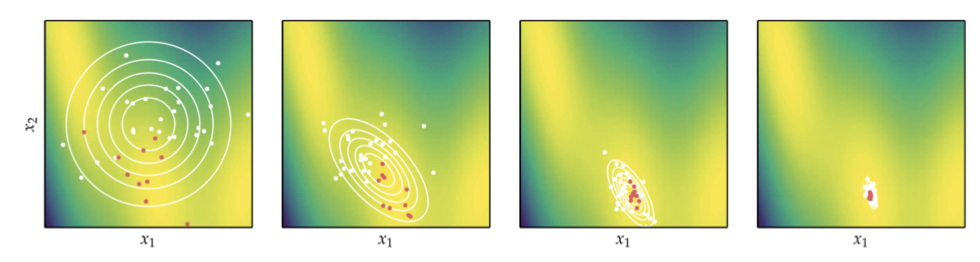
\includegraphics[width=120mm]{Figs/Cross-entropy.jpeg}
\end{figure}   
\end{frame}

\section{Covariance Matrix Adaptation}
\begin{frame}{Covariance Matrix Adaptation}
Covariance matrix adaptation maintains a mean vector $\boldsymbol{\mu}$, a covariance matrix $\boldsymbol{\Sigma}$, and an additional step-size scalar $\delta$. The covariance matrix only increases or decreases in a single direction with every iteration, whereas the step-size scalar is adapted to control the overall spread of the distribution. At every iteration, m designs are sampled from the multivariate Gaussian
\begin{equation*}
    \boldsymbol{x} \sim \mathcal{N} (\boldsymbol{\mu}, \sigma^2 \Sigma)
\end{equation*}

The designs are then sorted according to their objective function values such that $f(x^1) \leq f(x^2) \leq \cdots \leq f(x^m)$. A new mean vector  $\boldsymbol{\mu}^{k+1}$ is formed using a weighted average of the sampled designs:

\begin{gather*}
    \boldsymbol{\mu}^{k+1} \leftarrow \sum_{i=1}^m w_i \boldsymbol{x}^i\\
    \sum_i^m w_i = 1 ~~~~ w_1>w_2>\cdots>w_m>0    
\end{gather*}

\end{frame}

\begin{frame}{Covariance Matrix Adaptation}
The recommended weighting is obtained by
\begin{equation*}
    w`_i = \ln \frac{m+1}{2} - \ln i ~ \textrm{for~} i \in \{1, \cdots, m\}
\end{equation*}
to obtain $\boldsymbol{w} = \boldsymbol{w}`/\sum_i w`_i $.

The step size is updated using a cumulative $\boldsymbol{p}_\sigma$ that tracks steps over time
\begin{equation*}
    \begin{split}
        \boldsymbol{p}_\sigma^1 &= 0\\
        \boldsymbol{p}_\sigma^{k+1} &\leftarrow (1-c_\sigma)\boldsymbol{p}_\sigma + \sqrt{c_\sigma(2-c_\sigma)\mu_{\textrm{eff}}} (\Sigma^k)^{-1/2} \sigma_w \\
        \mu_{\textrm{eff}} &= \frac{1}{\sum_i w^2_i}\\
        \sigma_w &= \sum_{i=1}^{m_{\textrm{elite}}} 
        w_i \sigma^i ~ \textrm{for~} \sigma^i = \frac{\boldsymbol{x}^i - \boldsymbol{\mu}^k}{\sigma^k}
    \end{split}
\end{equation*}
\end{frame}

\begin{frame}{Covariance Matrix Adaptation}
The new step size is 
\begin{equation*}
    \sigma^{k+1} \leftarrow \sigma^k \exp\bigg(\frac{c_\sigma}{d_\sigma} \bigg[\frac{||\boldsymbol{p}_\sigma
    ||}{\mathbb{E}||\mathcal{N}(0, \boldsymbol{I})||}-1\bigg]\bigg)
\end{equation*}
where $\mathbb{E}$ is the expected length of a vector drawn from Gaussian distribution.
\begin{equation*}
    \mathbb{E}||\mathcal{N}(0, \boldsymbol{I})|| = \sqrt{2} \frac{\Gamma(\frac{n+1}{2})}{\Gamma(\frac{n}{2})}
    \approx \sqrt{n}\bigg(1-\frac{1}{4n}+\frac{1}{21n^2}\bigg)
\end{equation*}

\begin{equation*}
    \begin{split}
    c_\sigma &= (\mu_{\textrm{eff}}+2)/(n+\mu_{\textrm{eff}}+5)\\
    d_\sigma &= 1 + 2\max (0, \sqrt{\mu_{\textrm{eff}}-1)/(n+1)} -1 ) + c_\sigma         
    \end{split}
\end{equation*}

\end{frame}

\begin{frame}{Covariance Matrix Adaptation}
The covariance matrix is updated as follows
\begin{equation*}
    \begin{split}
    \boldsymbol{p}_\Sigma^1 &= 0\\
    \boldsymbol{p}_\Sigma^{k+1} &\leftarrow (1-c\Sigma)\boldsymbol{p_\Sigma^k} + h_\sigma \sqrt{c\Sigma (2-c_\Sigma) \mu_{\textrm{eff}}}\boldsymbol{\sigma}_w
    \end{split}
\end{equation*}

where 
\begin{equation*}
    h_\sigma =
    \begin{cases}
    1& if \frac{||\boldsymbol{p}_\Sigma||}{(1-c_\sigma^{2k+1})} < (1.4 + \frac{2}{n+1})  \mathbb{E}||\mathcal{N}(0, \boldsymbol{I})||\\
    0& \textrm{otherwise}
    \end{cases}
\end{equation*}

The update requires the adjusted weights $\boldsymbol{w}$:

\begin{equation*}
    w_i^0 =
    \begin{cases}
    w_i& \textrm{if~} w_i \geq 0 \\
    \frac{nw_i}{||\Sigma^{-1/2}\boldsymbol{\delta}^i||^2}& \textrm{otherwise}
    \end{cases}
\end{equation*}

\end{frame}

\begin{frame}{Covariance Matrix Adaptation}
The The covariance update is then
\begin{equation*}
    \Sigma^{k+1} \leftarrow [1 + c_1 c_\sigma(1-h_\sigma)(2 - c_\sigma) - c_1 - c_\mu]\Sigma^k 
    + c_1 \boldsymbol{p}_\Sigma \boldsymbol{p}_\Sigma^T + c_\mu \sum_{i=1}^\mu w_i^0 \boldsymbol{\delta}^i (\boldsymbol{\delta}^i)^T
\end{equation*}

The constants have the following recommended values
\begin{equation*}
    \begin{split}
    c_\Sigma &= \frac{4+\mu_{\textrm{eff}}/n}{n+4+2\mu_{\textrm{eff}}/n}\\
    c_1 &= \frac{2}{(n+1.3)^2 + \mu_{\textrm{eff}}} \\
    c_\mu &= \min \bigg( 1-c_1,  2\frac{\mu_{\textrm{eff}}-2+1/\mu_{\textrm{eff}}} {(n+2)^2 + \mu_{\textrm{eff}} } \bigg)
    \end{split}
\end{equation*}

\end{frame}

\begin{frame}{Covariance Matrix Adaptation}
\begin{figure}
\centering
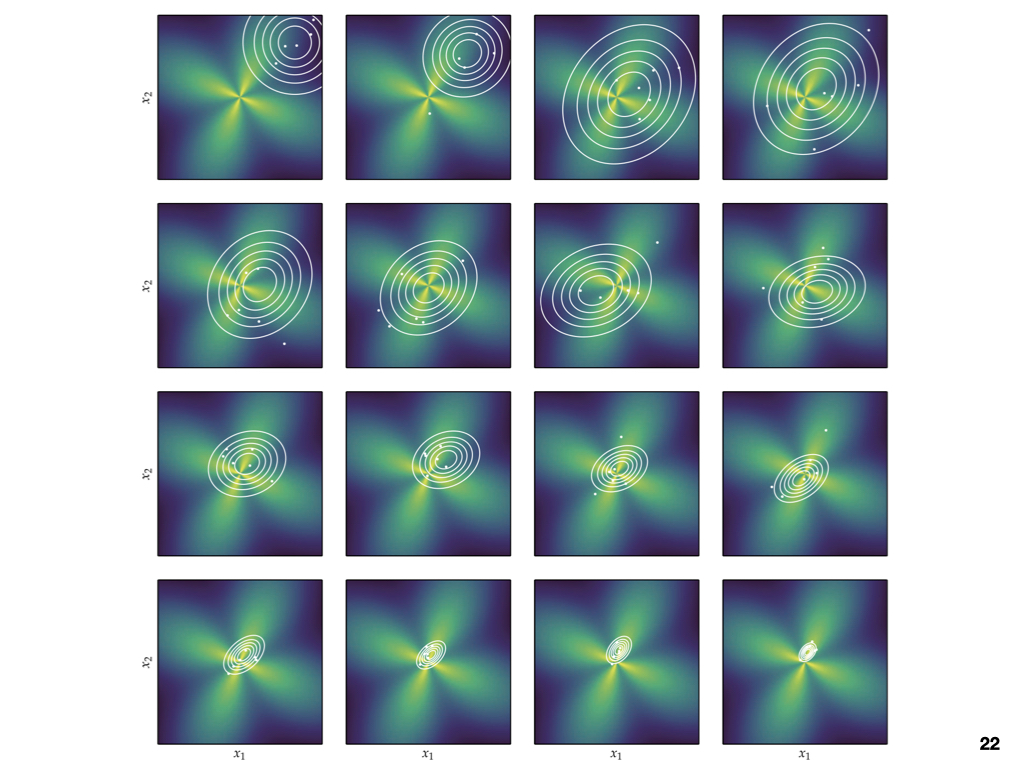
\includegraphics[width=100mm]{Figs/CMA.jpeg}
\end{figure}   
\end{frame}


\section{Summary}
\begin{frame}{Summary}
    \begin{itemize}
        \item Stochastic methods employ random numbers during the optimization process
        \item Simulated annealin guses a temperature that controls random exploration and which is reduced over time to converge on a local minimum.
        \item The cross-entropy method and evolution strategies maintain proposal distributions from which they sample in order to inform updates.
        \item Covariance matrix adaptation is a robust and sample-efficient optimizer that maintains a multivariate Gaussian proposal distribution with a full covariance matrix.
    \end{itemize}
\end{frame}
\end{document}

